\documentclass{article}
\usepackage[T1]{fontenc}
\usepackage{titlesec}
\usepackage{graphicx}
\usepackage{amsmath}
\usepackage{xcolor}
\usepackage{amssymb}
\usepackage{circuitikz}
\usepackage{trace}
\titleformat{\section}  % which section command to format
  {\fontsize{10}{12}\bfseries} % format for whole line
  {\thesection} % how to show number
  {1em} % space between number and text
  {} % formatting for just the text
  [] % formatting for after the text
  \title{Logika Cyfrowa}
\author{Jakub Gałaszewski} 
\begin{document}
\maketitle
\section{Zaprojektuj 3-bitowy licznik synchroniczny z ładowaniem równoległym przy użyciu przerzutników typu T.}
\textbf{licznik synchroniczny} to licznik którego każdy przerzutnik jest zsynchronizowany z zegarem, dzięki czemu nie ma żadnych opóźnień.\\
\begin{center}
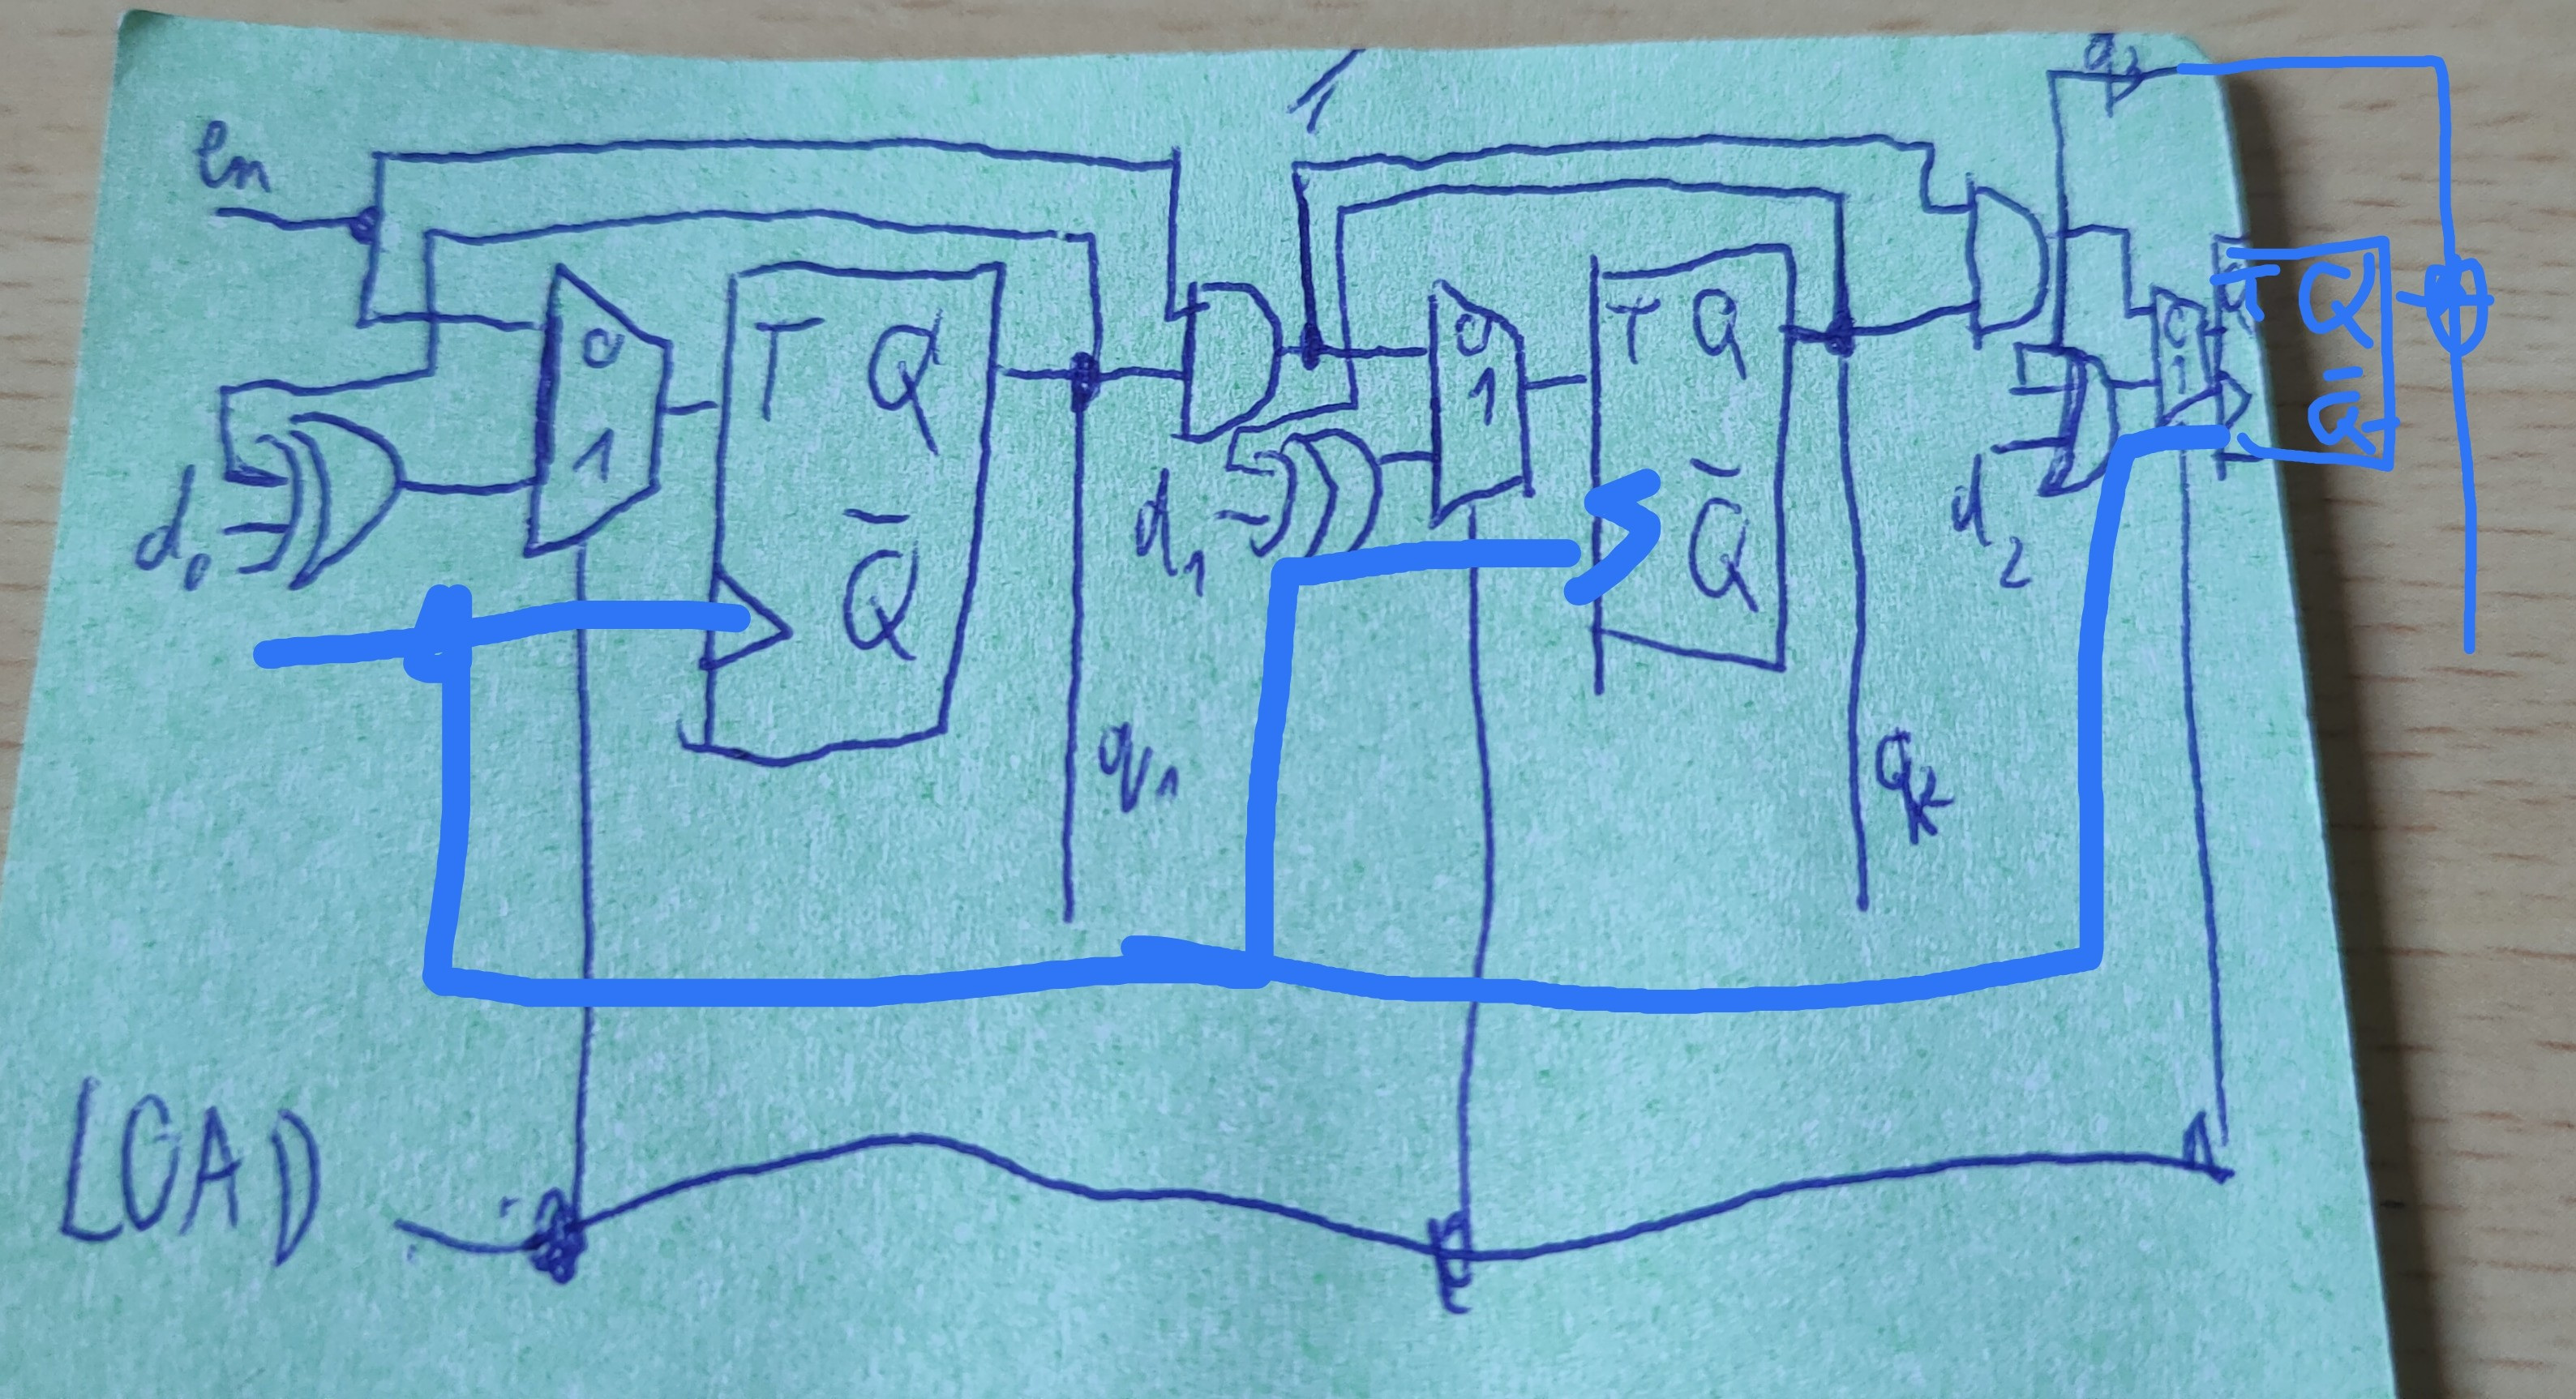
\includegraphics[scale=0.1]{./L07Z01.jpg}
\end{center}
\section{Zaprojektuj 3-bitowy licznik synchroniczny odliczający w górę lub w dół, wykorzystujący przerzutniki typu T. Układ powinien zawierać wejście ~up/down.}
\begin{center}
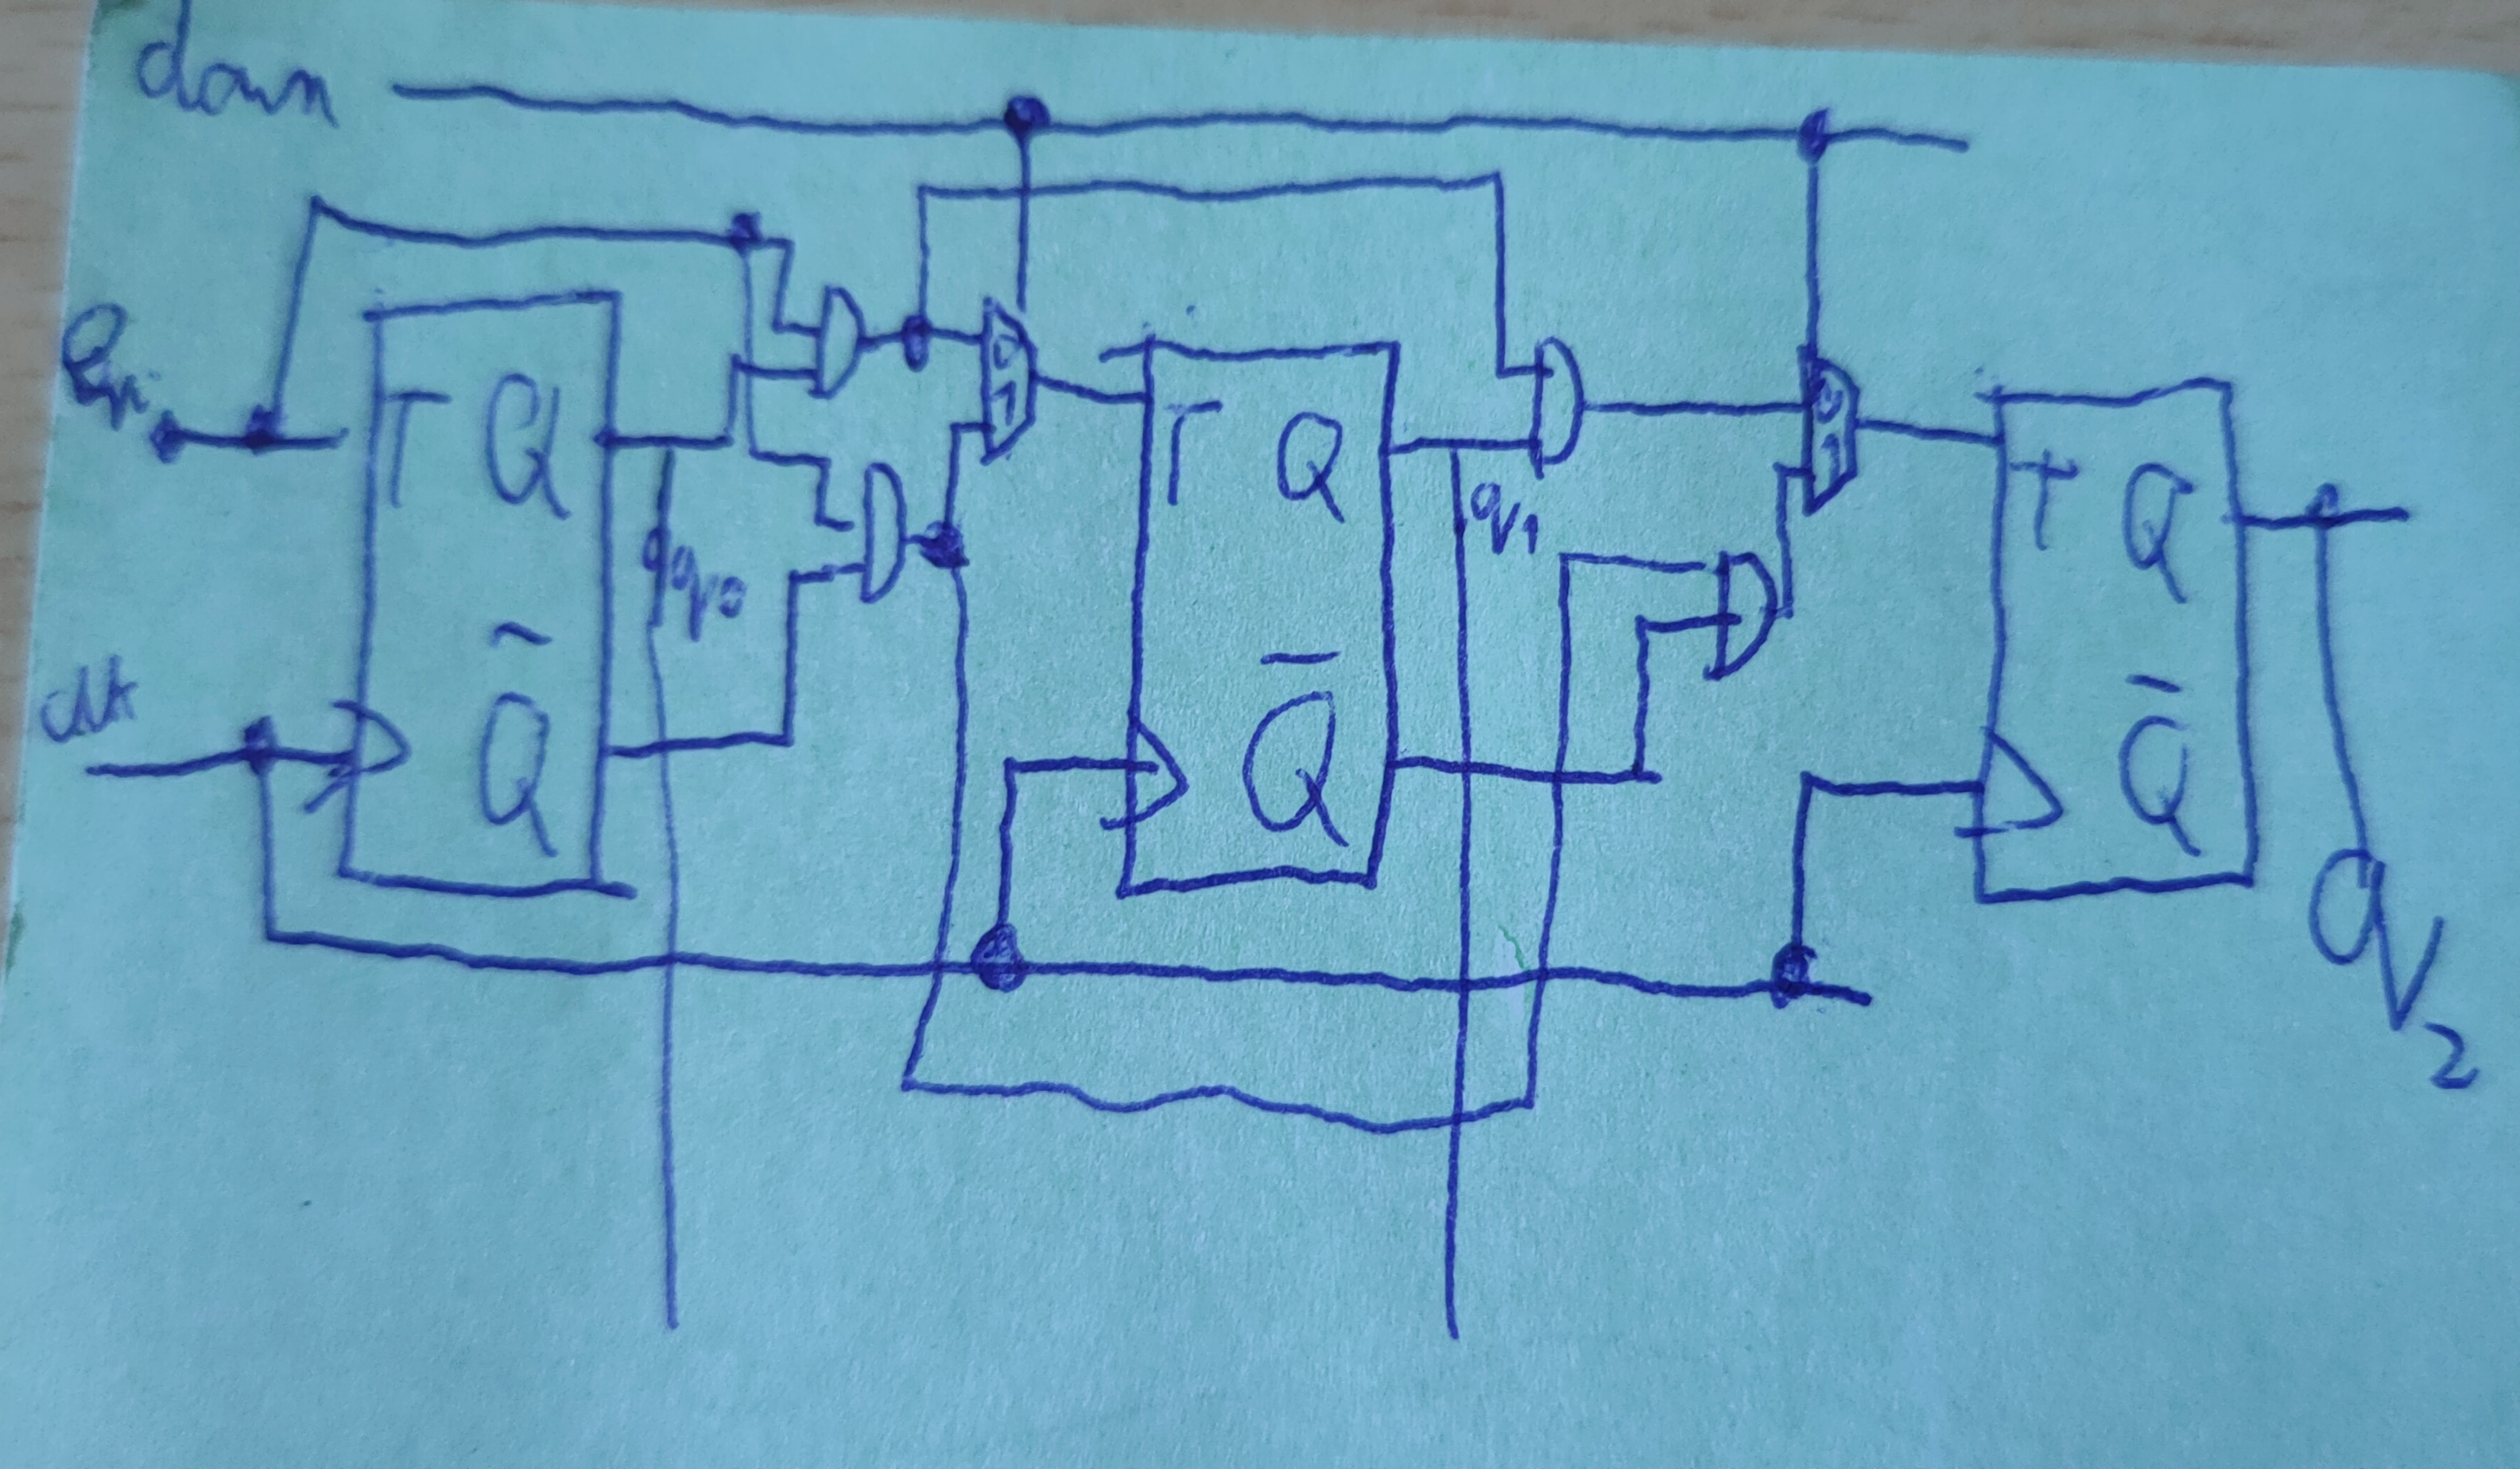
\includegraphics[scale=0.07]{./L07Z02.jpg}
\end{center}
\section{Poniższy układ wygląda jak licznik. Jak wygląda jego sekwencja odliczania?}
\begin{center}
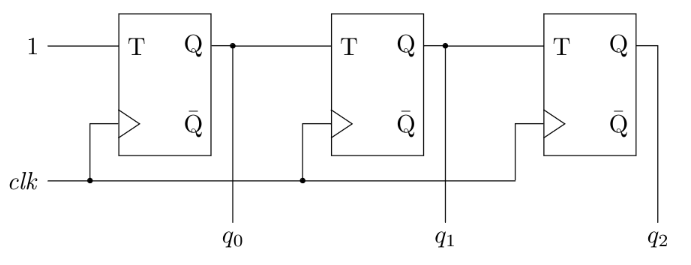
\includegraphics[scale=0.4]{./L07Z03.png}
\end{center}
0-1-2-7-0\\ ($000$, $100$, $010$, $111$, $000$)\\
3-4-5-6-3\\ ($110$, $001$, $101$, $011$, $110$)\\

\section{}
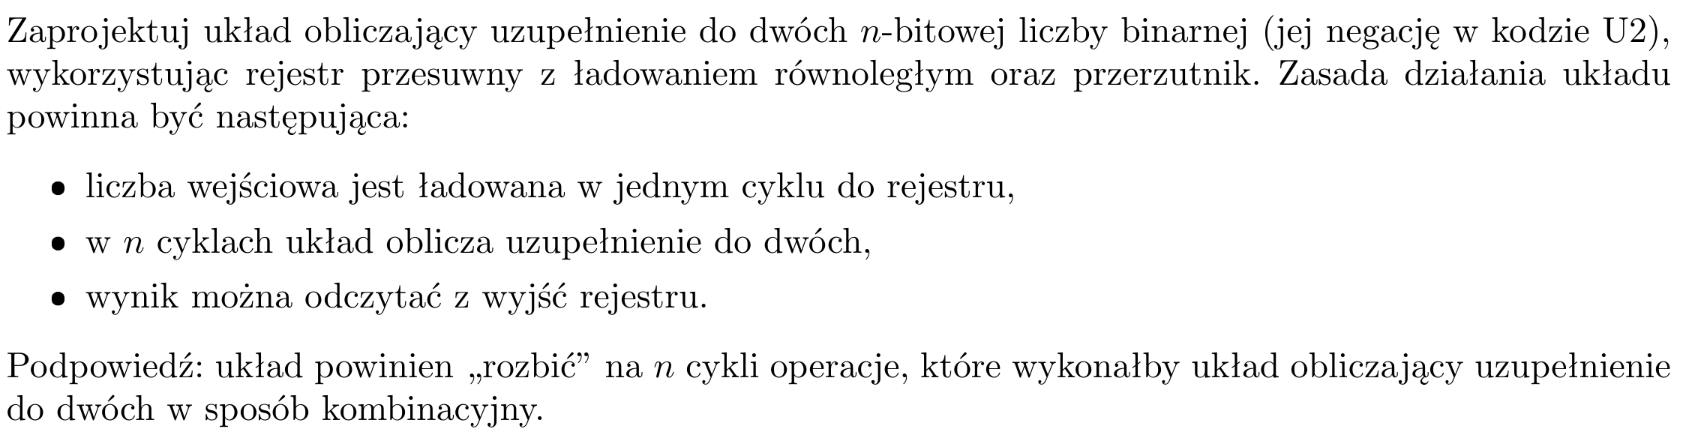
\includegraphics[scale=0.3]{./L07Z04.png}
\begin{center}
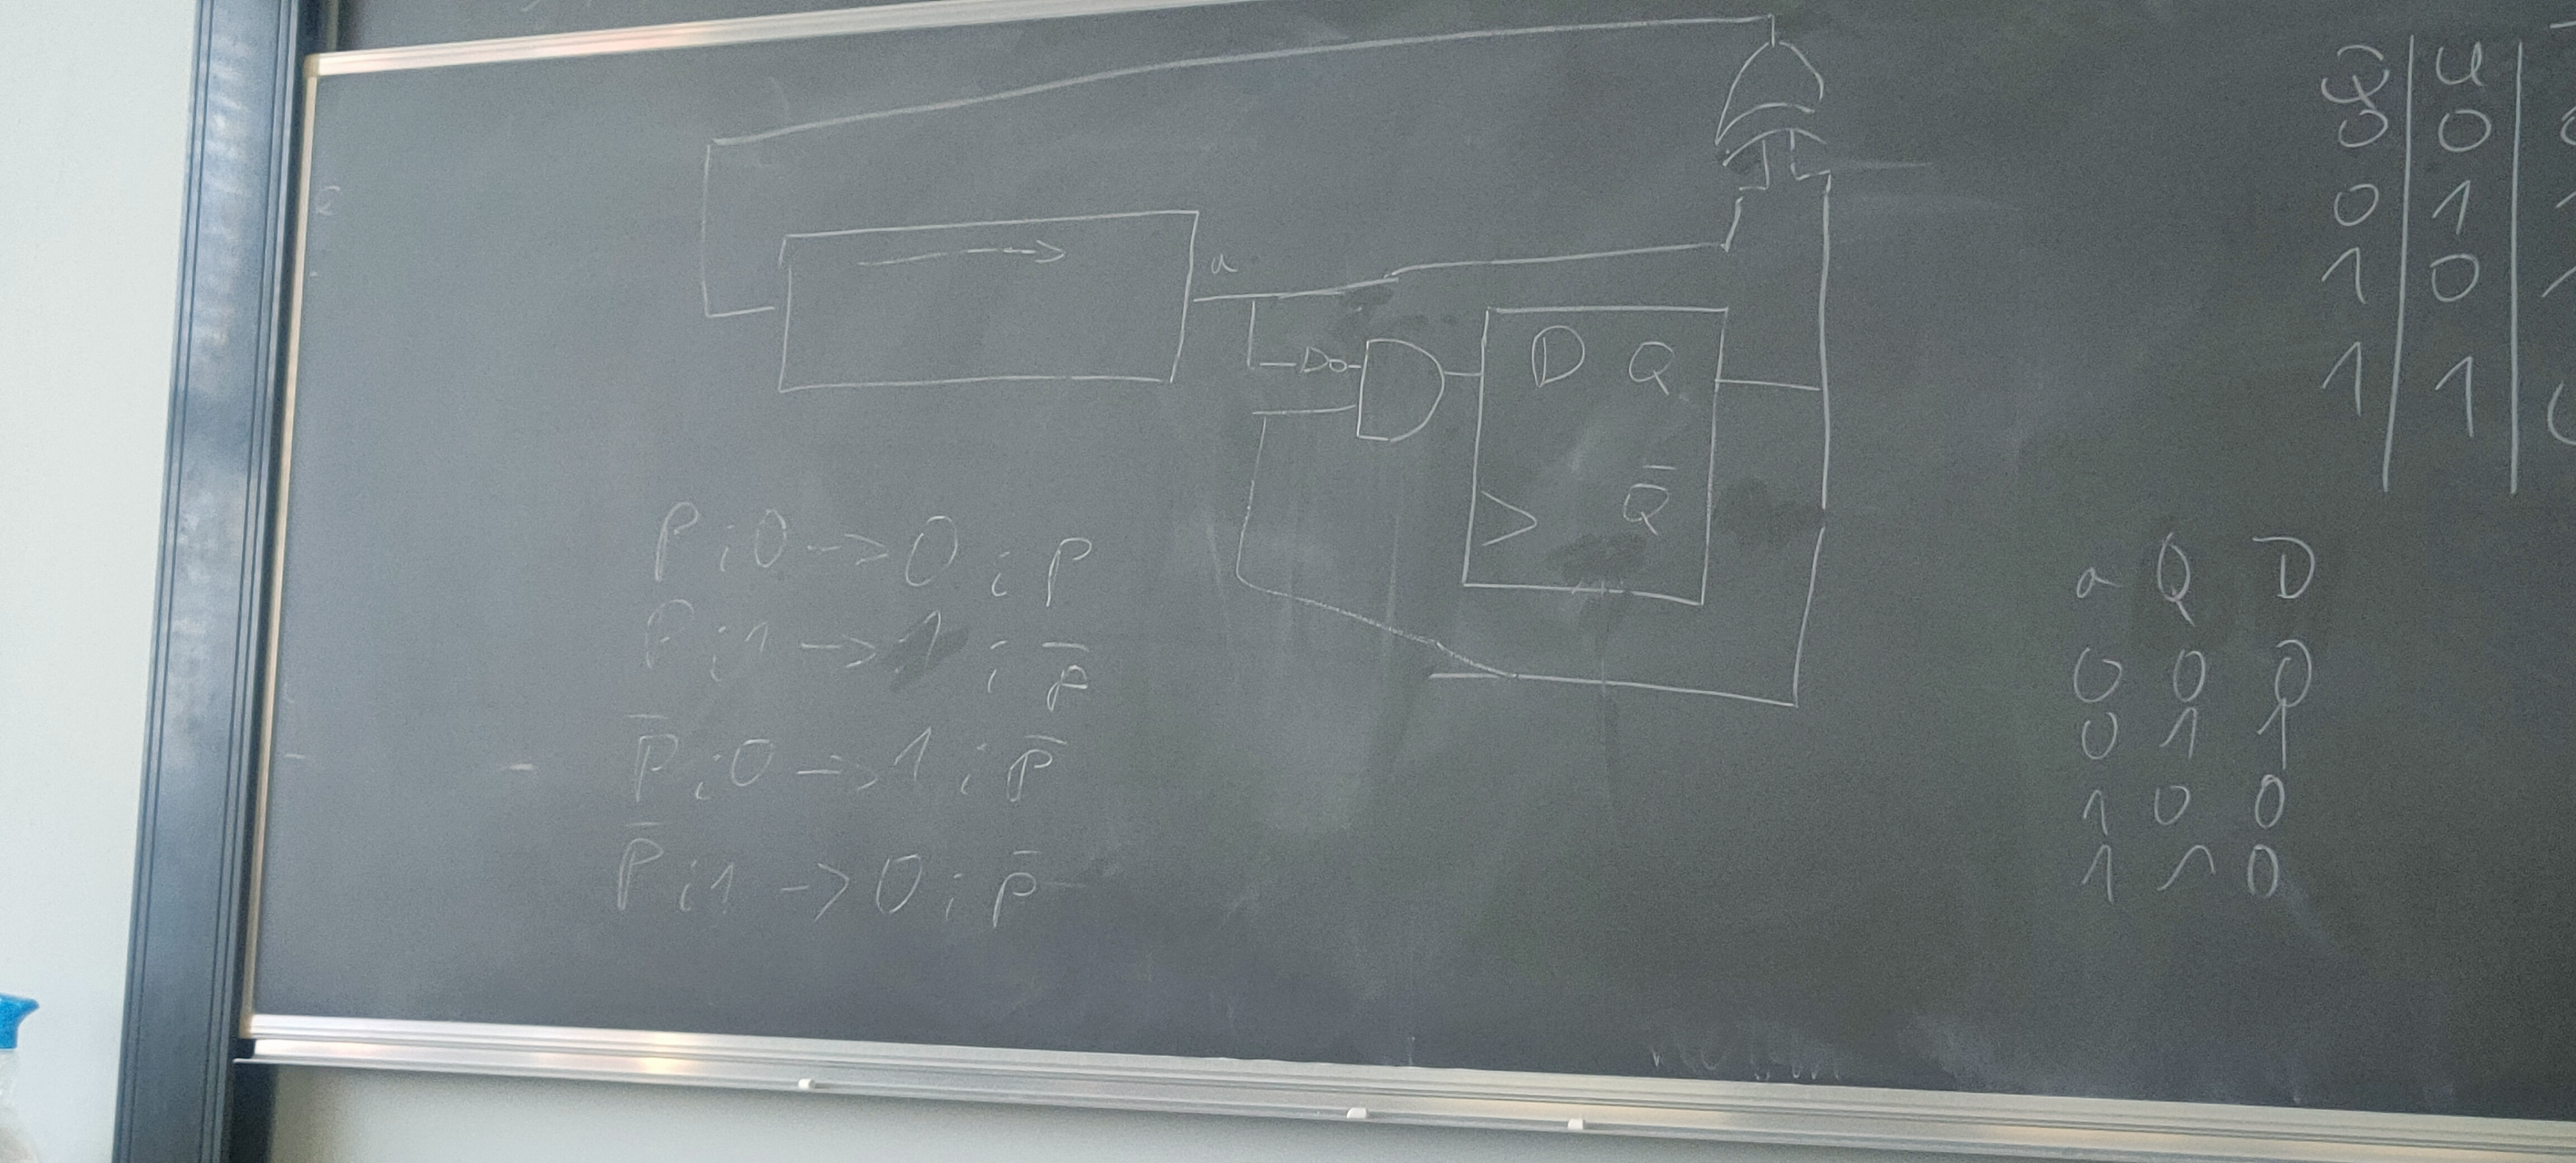
\includegraphics[scale=0.05]{./L07Z04.jpg}
\end{center}

\section{ednocyfrowy licznik BCD z wykładu posiada 6 nieużywanych stanów. Określ, jaki będzie kolejny stan licznika dla każdego z tych stanów. Co się stanie, jeśli z powodu usterki układ znajdzie się w jednym z nich?}
\begin{center}
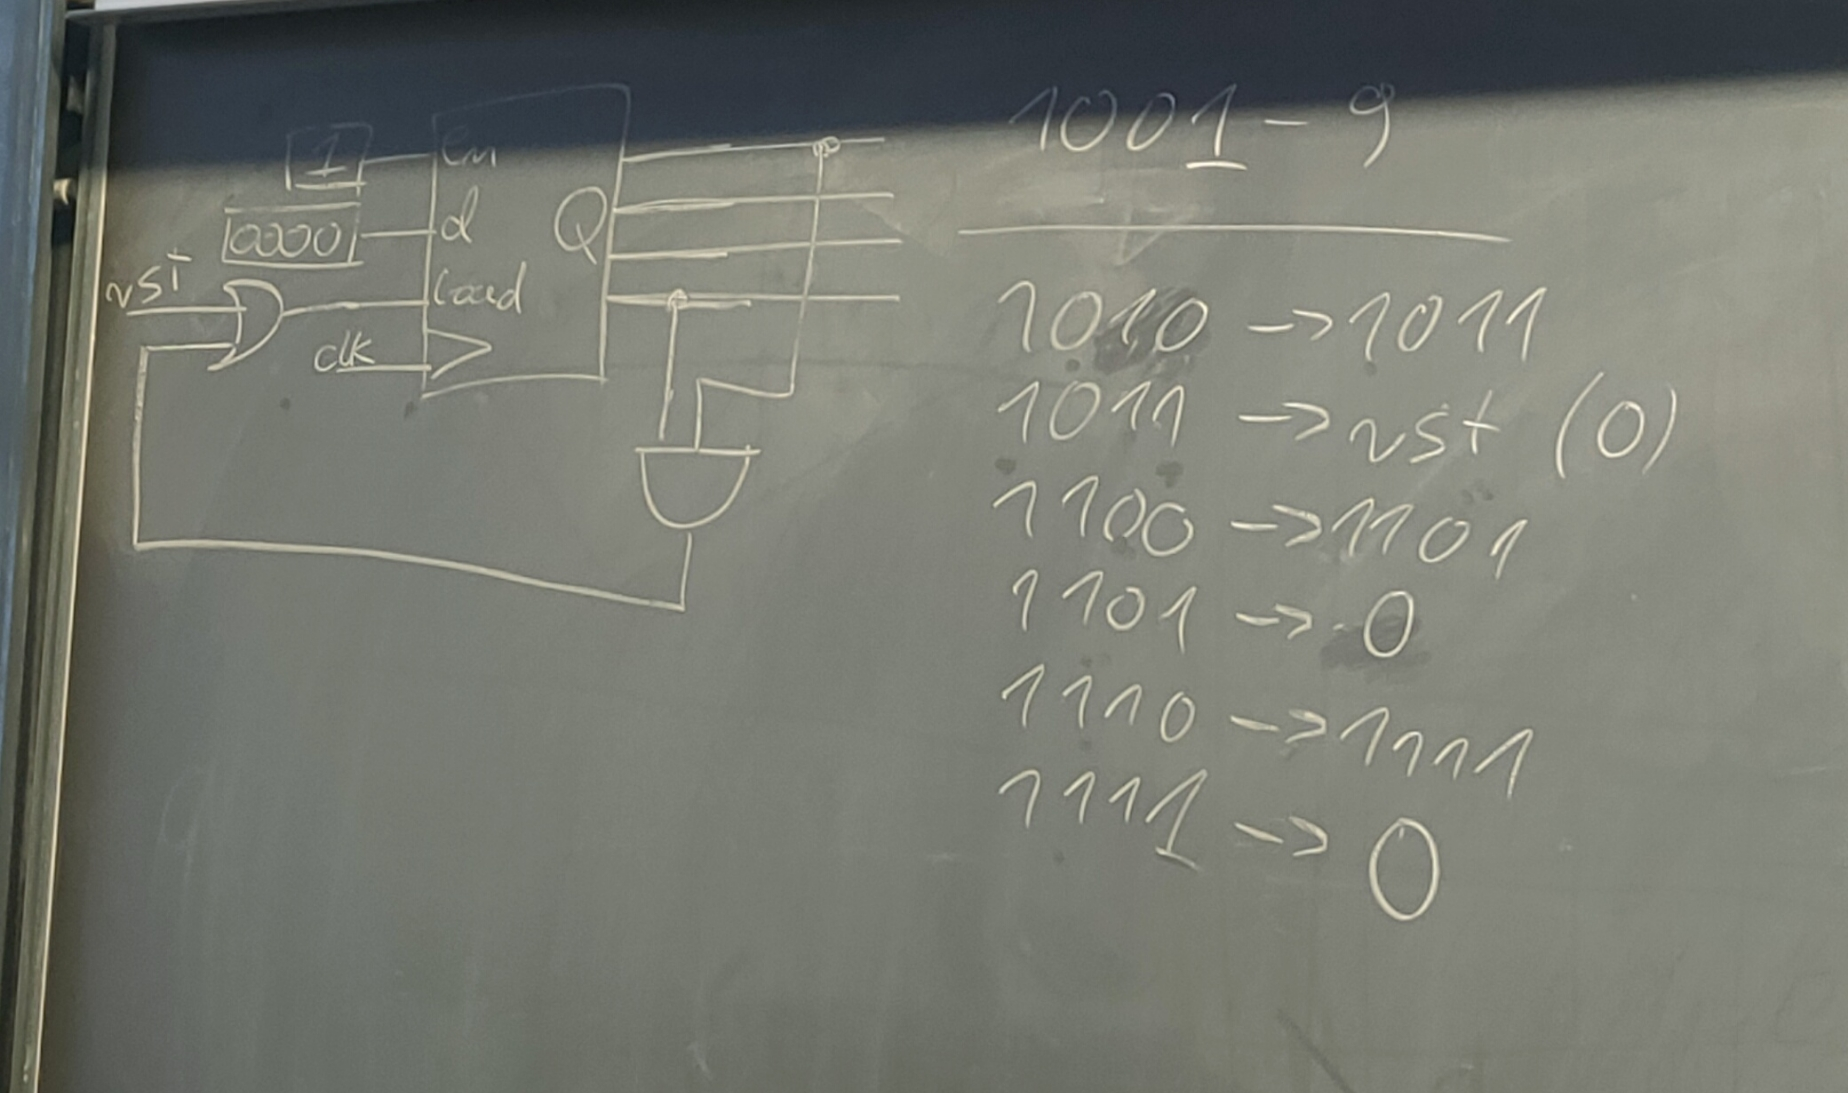
\includegraphics[scale=0.2]{./L07Z05.jpg}
\end{center}
\section{Zaprojektuj obwód, który, po otrzymaniu sygnału startowego, wygeneruje na swoim wyjściu stan wysoki przez dokładnie 12 cykli, po czym zmieni stan wyjścia na niski. Wyjście powinno pozostać w stanie niskim do pojawienia się kolejnego sygnału startowego.}
\begin{center}
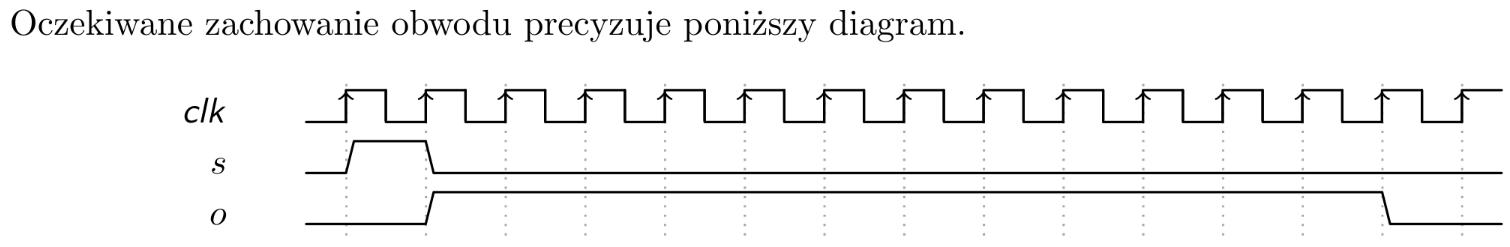
\includegraphics[scale=0.3]{./L07Z06.png}
\\
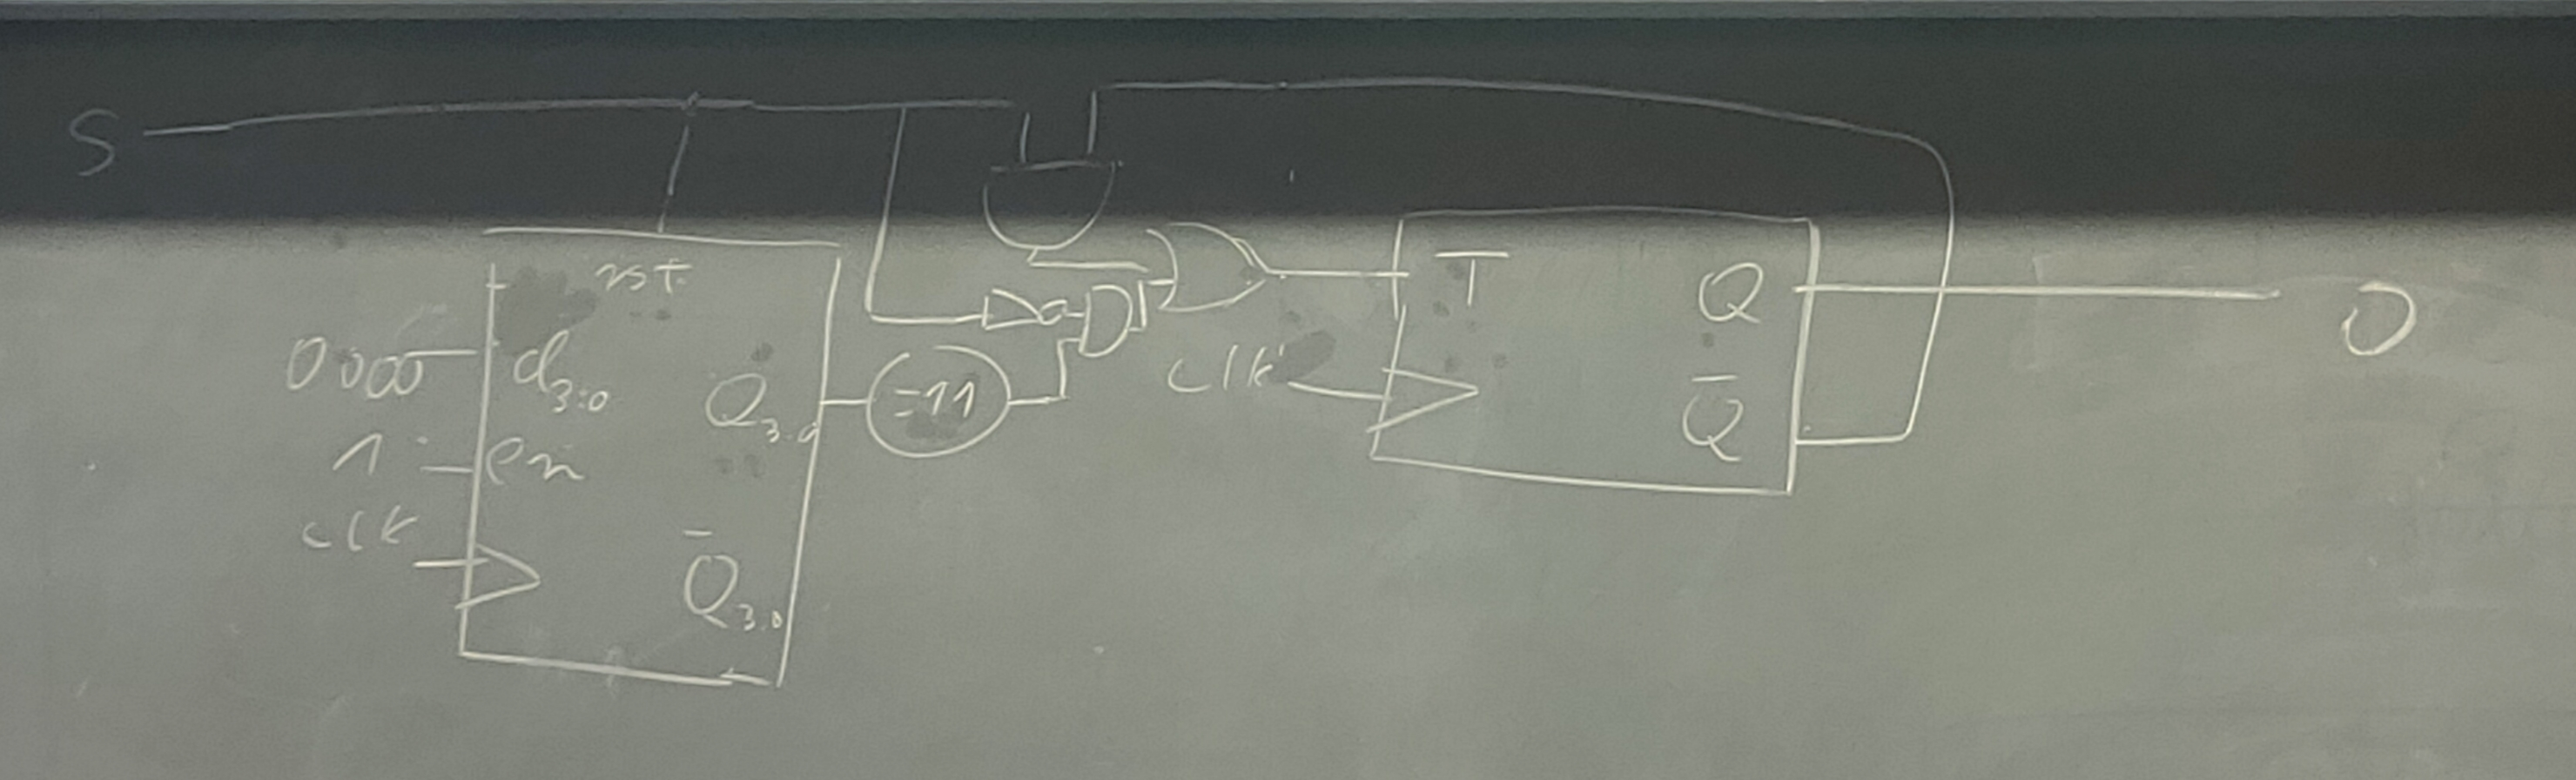
\includegraphics[scale=0.1]{./L07Z06v1.jpg}
\\
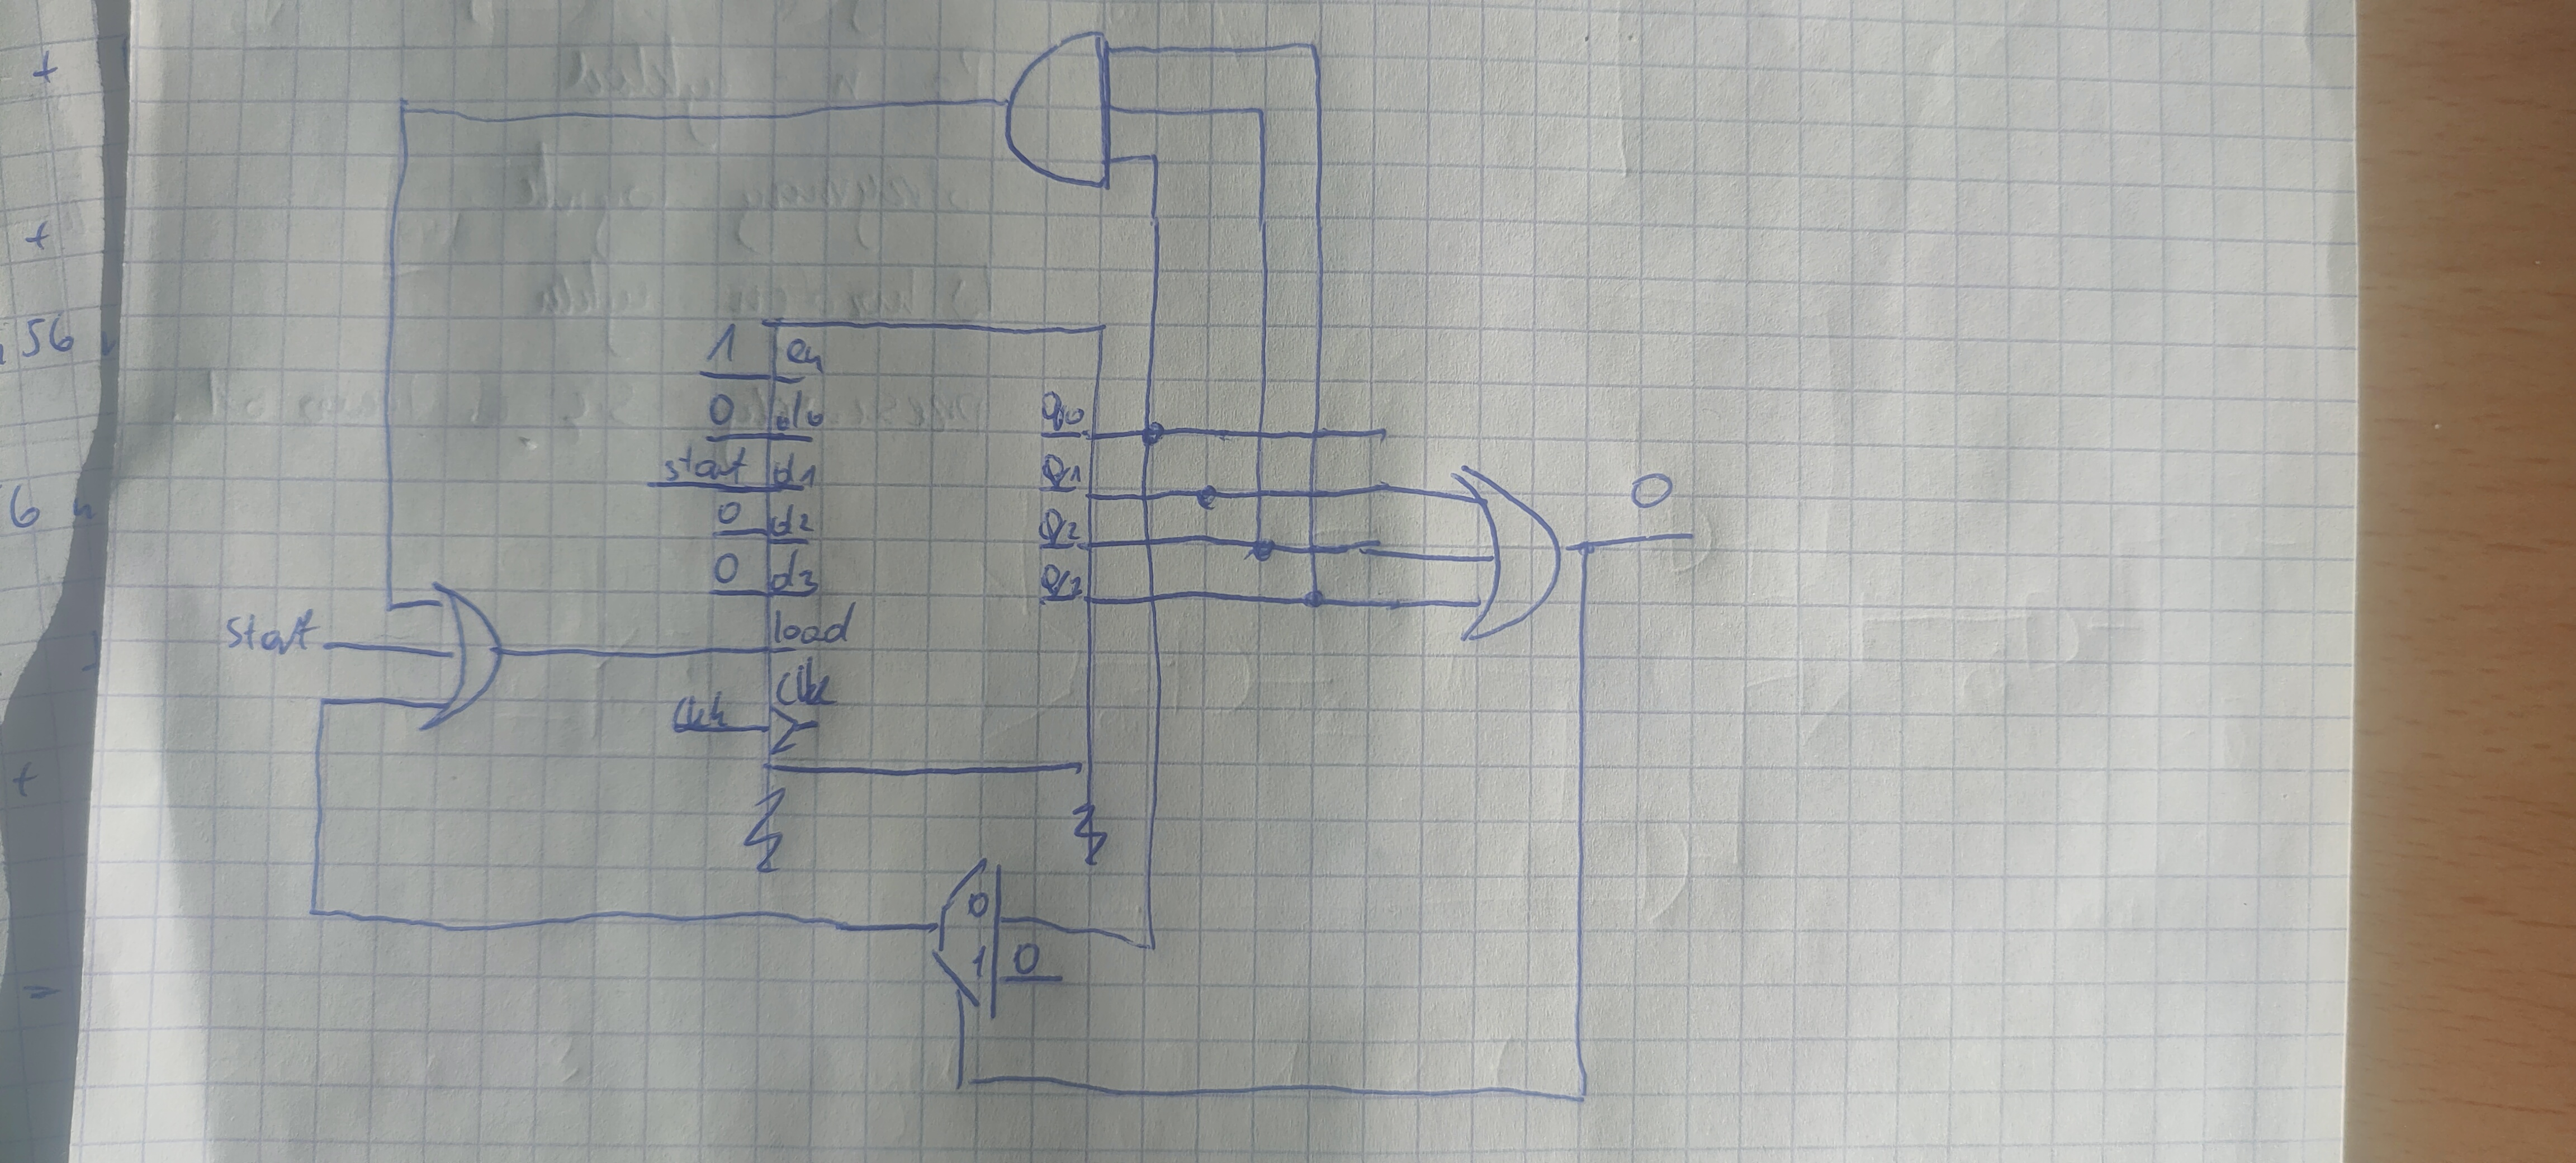
\includegraphics[scale=0.05]{./L07Z06v2.jpg}
\end{center}
\section{Dla licznika synchronicznego z ładowaniem równoległym pokazanego na wykładzie wyznacz maksymalną częstotliwość zegara, zakładając czasy propagacji i czas ustalania przerzutnika podane na wykładzie:}
$t^{dff}_p = 44 ns$\\
$t^{and}_p = t^{or}_p = 23 ns$\\
$t^{xor}_p = 30 ns$\\
$t^{dff}_{su} = 20 ns$\\
aby obliczyć czas, należy przejść od wyjścia dowolnego przerzutnika do wejścia dowolnego przerzutnika.\\
\begin{center}
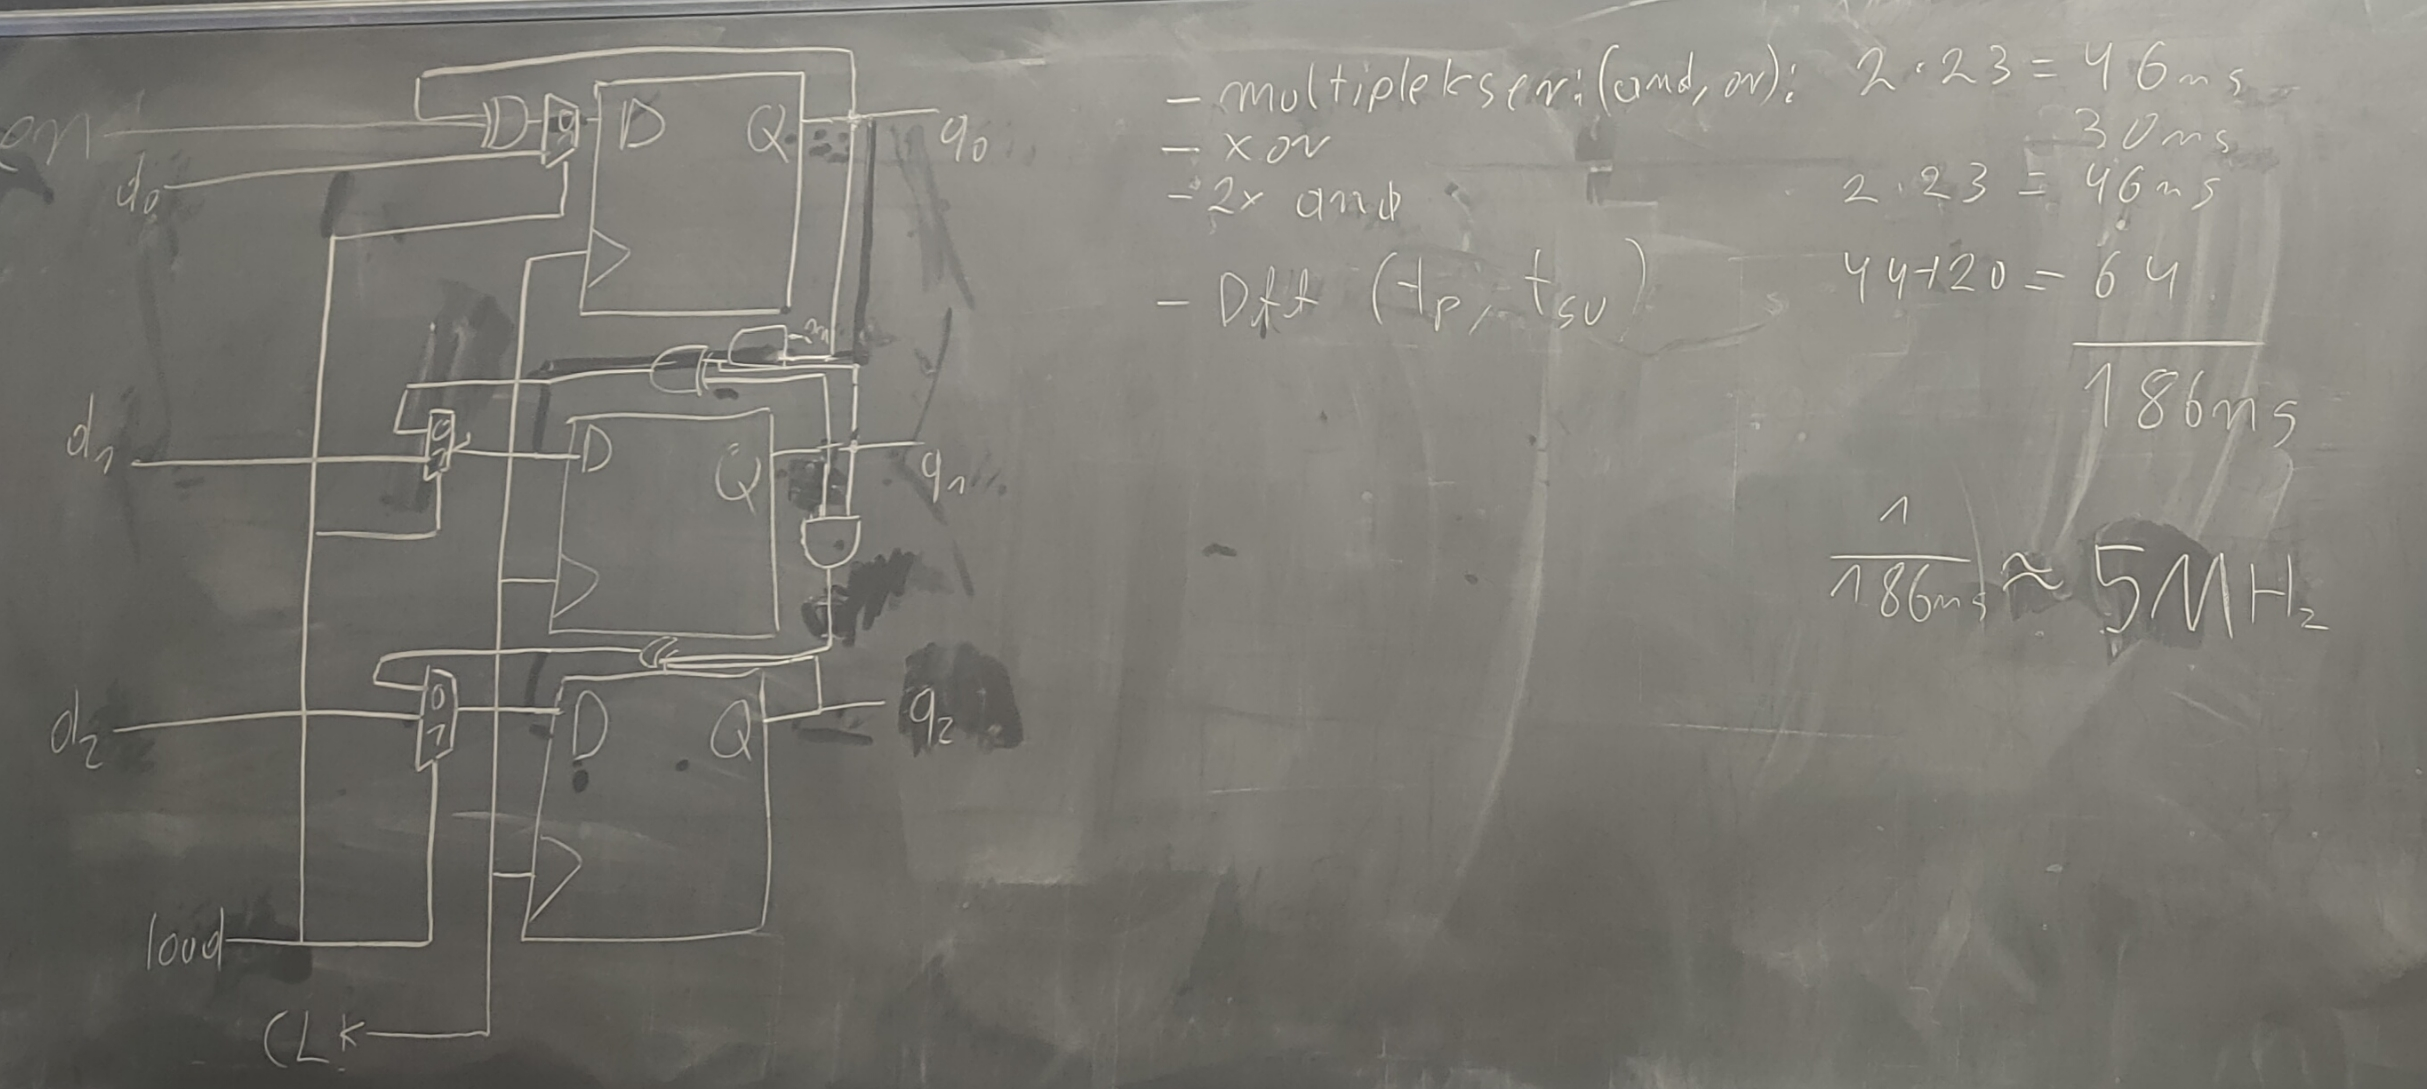
\includegraphics[scale=0.1]{./L06Z07.jpg}
\end{center}

\end{document}